\documentclass{beamer}

% Copyright 2010 Drow Ltd.
% 
% In principle, this file can be redistributed and/or modified under
% the terms of the GNU Public License, version 2.
% 
% However, this file is supposed to be a template to be modified
% for your own needs. For this reason, if you use this file as a
% template and not specifically distribute it as part of a another
% package/program, I grant the extra permission to freely copy and
% modify this file as you see fit and even to delete this copyright
% notice. 
\mode<presentation>
{
  \usetheme[titleline=true,
  alternativetitlepage=true,
  titlepagelogo=images/Java_logo]{Torino}
  \usecolortheme{nouvelle}
  \beamertemplatenavigationsymbolsempty
}

\usepackage{times}
\usepackage[utf8]{inputenc}
\usepackage[english,bulgarian]{babel}
\usepackage[T2A]{fontenc}

\usepackage{listings}
\lstset{language=Java,
  captionpos=b,
  tabsize=4,
  keywordstyle=\color{blue},
  commentstyle=\color{gray},
  stringstyle=\color{green},
  numbers=left,
  breaklines=true,
  showstringspaces=false,
  basicstyle=\ttfamily,
  emph={label},
  frame=shadowbox, 
  rulesepcolor=\color{blue},
  columns=fixed}

\title{Въведение в платформата за програмиране Java}

\author{инж. Божидар Бацов}

\institute{Drow Ltd.}

\date{26.10.2010}

\subject{Talks}
% This is only inserted into the PDF information catalog. Can be left
% out. 

% show toc at the beginning of each section
\AtBeginSection[]
{
  \begin{frame}<beamer>{Съдържание}
    \tableofcontents[currentsection,currentsubsection]
  \end{frame}
}

\begin{document}

\begin{frame}
  \titlepage
\end{frame}

\begin{frame}{Съдържание}
  \tableofcontents[pausesections]
\end{frame}

\section{За курса}

\begin{frame}{Екип}
  \transdissolve
  \begin{itemize}
  \item инж. Божидар Бацов
    \begin{itemize}
    \item Технически директор на Drow Ltd.
    \item Професионален софтуерен инженер
    \item Професионален системен администратор
    \item Ентусиаст на тема програмиране, GNU/Linux, Emacs и свободен
      софтуер
    \item Бездарен китарист, пенсиониран gamer, кинокритик на свободна
      практика
    \end{itemize}
    \pause
  \item Владимир Василев
    \begin{itemize}
      \item Благ диктатор на init Lab
      \item Професионален софтуерен инженер
      \item Професионален кейтърър
      \item Радетел за свободен софтуер, свободни технологии
    \end{itemize}
  \end{itemize}
\end{frame}

\begin{frame}{Комуникация}
  \transdissolve
  \begin{itemize}
  \item Пощенски списък 
    \begin{itemize}
    \item http://groups.google.com/group/java-in-action
    \item http://groups.google.com/group/init-lab
    \end{itemize}
    \pause
  \item Електронна поща
    \begin{itemize}
      \item bozhidar.batsov@gmail.com
      \item vlood.vassilev@gmail.com
    \end{itemize}
    \pause
  \item Jabber/GTalk
    \pause
  \item Twitter
    \begin{itemize}
      \item bbatsov
      \item initLabber
    \end{itemize}
    \pause
  \item Facebook група Java in Action
  \end{itemize}
\end{frame}

\begin{frame}{Формат на занятията}
  \transdissolve
  \begin{itemize}
  \item Лекции по 45 минути
  \item Почивки по 15 минути
  \item Задачки-закачки за упражнение
  \item Допълнителни практически занятия
  \item Работа по учебен проект
  \end{itemize}
\end{frame}

\begin{frame}{Защо е добра идея човек да научи Java?}
  \transdissolve
  \begin{itemize}
    \item 4.5 милиарда устройства използват Java \pause
      \begin{itemize}
        \item 850+ милиона персонални компютри \pause
        \item 2.1 милиарда мобилни телефони и устройства \pause
        \item 3.5 милиарда смарт карти \pause
        \item видео плеъри, игри, навигационни системи, банкови
          терминали, медицинска техника
      \end{itemize}
      \pause
    \item 6.5 милиона разработчици избраха Java, за да 
      \begin{itemize}
        \item пишат платформено независим софтуер, който работи на
          всяка процесорна архитектура и всяка операционна система \pause
        \item създават сървърни приложения и уеб услуги \pause
        \item разработват софтуер за телефони и други мобилни
          устройства \pause
      \end{itemize}
  \end{itemize}
\end{frame}

\begin{frame}{Програмирането}
  \transdissolve
  \textit{If art interprets our dreams, the computer executes them in the
  guise of programs!} \\
  \hskip 8cm \textbf{Alan J. Perlis}
  \pause
  \begin{itemize}
  \item Забавление \pause
  \item Предизвикателство за ума \pause
  \item Начин на живот \pause
  \item Професия \pause
  \item Черна магия \pause
  \item Алгоритми + структури от данни \pause
  \end{itemize}
\end{frame}

\begin{frame}{Програмистите}
  \transdissolve
  \begin{itemize}
  \item Сити(С програмисти) и Джедаи(Java програмисти) \pause
  \item Артисти и занаятчии \pause
  \item Качества на добрия програмист \pause
    \begin{itemize}
      \item Мързеливост \pause
      \item Нетърпеливост \pause
      \item Хюбрис(огромна гордост)
    \end{itemize}
  \end{itemize}
\end{frame}

\section{Платформата за програмиране Java}
\subsection{Програмирането преди ерата на Java}

\begin{frame}{Програмирането през 1995}
  \transdissolve
  \begin{itemize}
    \item C
    \item C++
    \item Lisp
    \item Pascal
    \item Smalltalk
  \end{itemize}
\end{frame}

\begin{frame}{Водещи езици в последните 25 години}
  \transdissolve
  \begin{tabular}{|c|c|c|c|c|}
    \hline
    Programming & Position & Position & Position & Position \\
    Language    & Oct 2010 & Oct 2005 & Oct 1995 & Oct 1985 \\
    \hline
    \hline
    Java        & 1        & 1        & 16       & -        \\
    \hline
    C           & 2        & 2        & 1        & 1        \\
    \hline
    C++         & 3        & 3        & 2        & 10       \\
    \hline
    PHP         & 4        & 4        & -        & -        \\
    \hline   
    (Visual) Basic & 5     & 6        & 3        & 4        \\
    \hline
    C\#         & 6        & 7        & -        & -        \\
    \hline
    Python      & 7        & 8        & 17       & -        \\
    \hline
    Objective-C & 8        & 44       & -        & -        \\
    \hline
    Perl        & 9        & 5        & 4        & -        \\
    \hline      
    Ruby        & 10       & 24       & -        & -        \\
    \hline 
    Lisp        & 13       & 14       & 8        & 2        \\
    \hline
    Ada         & 17       & 16       & 11       & 3        \\
    \hline
  \end{tabular}
\end{frame}

\subsection{Предимства на Java}
\begin{frame}{Предимствата на Java}
  \transdissolve
  \begin{itemize}
  \item Простота \pause
  \item Обектно-ориентирано програмиране \pause
  \item Архитектурна независимост \pause
  \item Портативност \pause
  \item Вградена мрежова поддръжка \pause
  \item Надеждност \pause
  \item Сигурност \pause
  \item Паралелизъм \pause
  \item Динамика
  \end{itemize}
\end{frame}

\begin{frame}{Простота}
  \transdissolve  
  \begin{itemize}
    \item Базиран на C++ \pause
    \item Изчистен синтаксис \pause
      \begin{itemize}
        \item няма указатели \pause
        \item няма презареждане на оператори \pause
        \item няма хедър(.h) файлове \pause
        \item няма структури(struct) - има само класове \pause
        \item няма unions
      \end{itemize}
      \pause
    \item Автоматично събиране на боклука(Garbage collection)
  \end{itemize}
\end{frame}

\begin{frame}{Обектно-ориентирано програмиране}
  \transdissolve
  \begin{itemize}
  \item Проектиран с ООП наум от самото начало \pause
  \item Усъвършенстван обектен модел от С++
  \end{itemize}
\end{frame}

\begin{frame}{Мрежова поддръжка и паралелизъм}
  \transdissolve
  \begin{itemize}
  \item Мрежова поддръжка
  \begin{itemize}
  \item Богата библиотека за работа с различни
    мрежови протоколи(TCP/IP, HTTP, FTP)
  \end{itemize}
  \pause
  \item Паралелизъм
    \begin{itemize}
    \item Вградена поддръжка за мултипроцесори
    \item Просто и гъвкаво API за работа с нишки
    \end{itemize}
  \end{itemize}
\end{frame}

\begin{frame}{Надеждност}
  \transdissolve
  \begin{itemize}
    \item Липсва на указатели и асоциираните с
    тях проблеми
    \begin{itemize}
      \item преливане на стека
      \item достъп до невалиден указател
    \end{itemize} 
    \pause
    \item Няма опасност от течове на памет - боклукчията 
    (garbage collector) се грижи за това
  \end{itemize}
\end{frame}

\begin{frame}{Сигурност}
  \transdissolve  
  \begin{itemize}
   \item Невъзможно е да прелее стека на
    изпълнение(runtime stack) \pause
   \item Невъзможно е да се наруши паметта
    извън собственото адресно
    пространство \pause
   \item Невъзможно е да се пишат/четат
    файлове без права
  \end{itemize}
\end{frame}

\begin{frame}{Преносимост}
  \transdissolve
  \begin{itemize}
  \item Стандартизирани типове
    \begin{itemize}
      \item byte = 1 byte
      \item short = 2 bytes
      \item int = 4 bytes
    \end{itemize}
    \pause
  \item Вградена поддръжка на различни
  файлови системи \pause
  \item Портативна библиотека за създаване на графични потребителски интерфейси
  \end{itemize}
\end{frame}

\begin{frame}{Висока производителност}
  \transdissolve
  \begin{itemize}
  \item Производителност близка до тази на
  приложения писани на C/C++ \pause
  \item Възможност за постигане на висока
  оптимизация на бинарния код по време
  на изпълнение
\end{itemize}
\end{frame}

\begin{frame}{Раждането на Java}
  \transdissolve
  \begin{itemize}
    \item Проектът Green и James Gosling \pause
    \item Езикът Oak \pause
    \item Изборът на името Java \pause
    \item Аплетите или началото на Java \pause
    \item Възходът на Java \pause
    \item Триумфът на Java
  \end{itemize}
\end{frame}

\begin{frame}{Програмен език номер 1 в света.}
  \transdissolve
  \begin{tabular}{|c|c|c|c|c|c|c|}
    \hline
    \textbf{Position} &
    \textbf{Position} & \textbf{Pos} & \textbf{Programming} &
    \textbf{Ratings} & \textbf{Delta} \\
    \textbf{Oct 2010} &
    \textbf{Oct 2009} & \textbf{Delta} & \textbf{Language} &
    \textbf{Oct 2010} & \textbf{2009} \\ 
    \hline
    \hline
    1 & 1 & = & Java & 18.166\% & -0.48\% \\
    \hline
    2 & 2 & = & C & 17.177\% & +0.33\% \\
    \hline
    3 & 4 & +1 & C++ & 9.802\% & -0.08\% \\
    \hline
    4 & 3 & -1 & PHP & 8.323\% & -2.03\% \\
    \hline
    5 & 5 & = & (Visual) Basic & 5.650\% & -3.04\% \\
    \hline
    6 & 6 & = & C\# & 4.963\% & +0.55\% \\
    \hline
    7 & 7 & = & Python & 4.860\% & +0.96\% \\
    \hline
    8 & 12 & +4 & Objective-C & 3.706\% & +2.54\% \\
    \hline
    9 & 8 & -1 & Perl & 2.310\% & -1.45\% \\
    \hline
    10 & 10 & = & Ruby & 1.941\% & -0.51\% \\
    \hline
  \end{tabular}
\end{frame}

\begin{frame}{Еволюцията на Java}
  \transdissolve
  \begin{tabular}{|c|c|c|c|}
    \hline
    \textbf{Версия} & \textbf{Година} & \textbf{Нововъведения в езика}
    & \textbf{Брой класове} \\
    & & & \textbf{и интерфейси} \\
    \hline
    1.0 & 1996 & Самият език & 211 \\
    \hline
    1.1 & 1997 & Вътрешни класове & 477 \\
    \hline
    1.2 & 1998 & Няма & 1524 \\
    \hline
    1.3 & 2000 & Няма & 1840 \\
    \hline
    1.4 & 2004 & Assertions & 2723 \\
    \hline
    5.0 & 2004 & Генерични класове, foreach, & 3279 \\ 
    & & varargs, autoboxing, metadata, & \\ 
    & & enumerations, static import & \\
    \hline
    6 & 2006 & Няма & 3777 \\
    \hline
  \end{tabular}
\end{frame}

\begin{frame}{Java и конкуренцията}
  \transdissolve
  \begin{itemize}
    \item Java срещу .NET и C\# \pause
    \item Java срещу C/C++ \pause
    \item Java срещу JavaScript \pause
    \item Java срещу Ruby/Python \pause
    \item Java срещу Groovy \pause
    \item Java срещу Scala \pause
    \item Java срещу Clojure
  \end{itemize}
\end{frame}

\subsection{Платформата Java}

\begin{frame}{Повече от език за програмиране}
  \transdissolve
  \begin{itemize}
    \item Език за програмиране \pause
    \item Среда за изпълнение на програми / Виртуална машина (JVM) \pause
    \item Пакет от инструменти за разработка на приложения (Java Dev
      Kit) \pause
  \end{itemize}

\end{frame}

\begin{frame}{Платформата Java}
  \transdissolve
  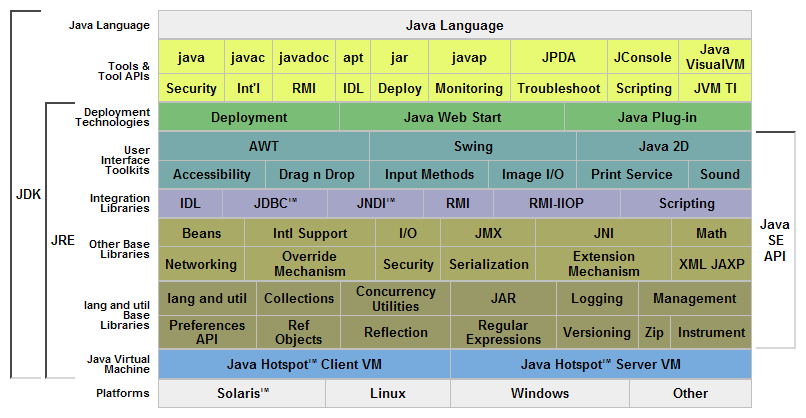
\includegraphics[height=200px, width=320px]{images/JavaPlatform.png}
\end{frame}

\begin{frame}{Java издания}
  \transdissolve
  \begin{itemize}
    \item Java Runtime Environment(JRE) \pause
    \item Java Development Kit(JDK) SE == JRE + dev tools \pause
    \item Java Enterprise Edition(Java EE) \pause
    \item Java Micro Edition(Java ME) \pause
  \end{itemize}
\end{frame}

\begin{frame}{Java имплементации}
  \transdissolve
  \begin{itemize}
  \item Различни дистрибутори
    \begin{itemize}
      \item Sun(Oracle) - Sun(Oracle) HotSpot VM, OpenJDK \pause
      \item IBM - IBM J9 \pause
      \item BEA Systems(Oracle) - JRockit \pause
      \item GNU - Classpath \pause
      \item Apache - Harmony 
    \end{itemize}
    \pause
  \item Референтна имплементация
    \begin{itemize}
      \item Oracle HotSpot VM
      \item Текуща версия - JDK 6 SE 1.6.0\_22
      \item Изтегляне от http://java.sun.com
    \end{itemize}
  \end{itemize}
\end{frame}

\section{Инсталиране на Java и първи стъпки}
\subsection{Инсталиране на JDK}
\begin{frame}{Инсталиране на Oracle JDK/OpenJDK}
  \transdissolve  
  \begin{itemize}
    \item Изтегляне на подходящ дистрибутив \pause
    \item Инсталиране под Линукс \pause
    \item Инсталиране под Уиндоус \pause
    \item Добавяне на изходния код и
      документацията на Java \pause
  \end{itemize}
\end{frame}

\subsection{Преглед на инструментите включени в JDK}
\begin{frame}{Основни инструменти}
  \transdissolve  
  \begin{itemize}
    \item \textbf{java} - стартира JVM
    \item \textbf{javac} - Java Compiler
    \item \textbf{jar} - инструмент за работа с jar архиви
    \item \textbf{javaws} - стартира Java Web Start
    приложение
    \item \textbf{jvisualvm} - много
    полезен графичен инструмент за следене на работата на JVM
  \end{itemize}
\end{frame}

\begin{frame}[fragile]
  \frametitle{Hey, Java!}
  \transdissolve
\begin{lstlisting}
public class HeyJava {
    public static void main(String[] args) {
        System.out.println("Hey, Java!");
    }
}
\end{lstlisting}
\end{frame}

\begin{frame}{Hey, Java!}
  \transdissolve  
  \begin{itemize}
    \item Създаваме файл HeyJava.java
    \item Създаваме в него прост клас HeyJava
    \item Запазваме файла
    \item Компилираме
      \begin{itemize}
        \item javac HeyJava.java
      \end{itemize}
    \item Стартираме
      \begin{itemize}
      \item java HeyJava
      \end{itemize}
  \end{itemize}
\end{frame}

\subsection{Интегрирани среди за разработка}
\begin{frame}{Интегрирани среди за разработка}
  \transdissolve  
  \begin{itemize}
    \item Интелигентен редактор \pause
    \item Анализ на кода \pause
    \item Интеграция с външния системи \pause
      \begin{itemize}
        \item инструмент за изграждане(build tool) \pause
        \item система за докладване на грешки(issue tracker) \pause
        \item система за управление на версиите(version control
          system) \pause
        \item интеграционнен сървър \pause
        \item други
      \end{itemize}
      \pause
    \item Интегриран дебъгер \pause
    \item Лесно рефакториране на кода
  \end{itemize}
\end{frame}

\begin{frame}{IntelliJ IDEA}
  \transdissolve
  \begin{itemize}
    \item Уеб сайт - www.jetbrains.com/idea
    \item Най-интелигентната среда за
    разработка на Java
    \item Консумира доста системни ресурси
    \item Две издания
      \begin{itemize}
        \item Ultimate - комерсиален продукт
        \item Community Edition - продукт с отворен код
      \end{itemize}
    \item Скромна документация, относително малка общност,
    малко разширения(plugins)
  \end{itemize}
\end{frame}

\begin{frame}{Eclipse}
  \transdissolve
  \begin{itemize}
    \item Уеб сайт - www.eclipse.org
    \item Най-използваната среда за разработка
    \item Голяма общност, безброй разширения
    \item По-скоро платформа, върху която да се
    изгражда софтуер, отколкото Java IDE
    \item Тромова система за работа с
    разширения, ниско качество на много
    разширения
  \end{itemize}
\end{frame}

\begin{frame}{NetBeans}
  \transdissolve  
  \begin{itemize}
    \item Уеб сайт - www.netbeans.org
    \item “Официалната” среда за разработка на
    Java приложения
    \item Лесен за използване, голяма общност
    \item Платформа за изграждане на приложения(NetBeans RCP)
    \item Най-добрата поддръжка на някои Sun-
    centric технологии
  \end{itemize}
\end{frame}

\begin{frame}[fragile]
  \frametitle{Swing пример}
  \transdissolve
\begin{lstlisting}[basicstyle=\tiny]
import javax.swing.*;
import java.awt.event.*;

public class HeySwing {
  public static void main(String[] args) {
    final JFrame frame = new JFrame();
    frame.setTitle("Java Rules!");
    frame.setSize(200, 200);

    JButton button = new JButton("Press me");
    button.addActionListener(new ActionListener() {
      @Override
      public void actionPerformed(final ActionEvent e) {
        JOptionPane.showMessageDialog(frame, "Swing power!");
      }
    });

    frame.add(button);
    frame.setDefaultCloseOperation(JFrame.EXIT_ON_CLOSE);

    frame.setVisible(true);
    }
}
\end{lstlisting}
\end{frame}

\begin{frame}{Демонстрация на IntelliJ IDEA}
  \transdissolve
  \begin{itemize}
    \item Създаване на Java проект
    \item Създаване на просто Java приложение
    \item Стартиране на приложението
  \end{itemize}
\end{frame}

\section{GitHub}
\begin{frame}{Системи за управление на изходния код}
  \transdissolve
  \begin{itemize}
  \item Основни характеристики
    \begin{itemize}
      \item позволяват работата на група хора върху файлове на проекта
      \item история на промените
      \item отмяна на промени
      \item алтернативни клонове на разработка
    \end{itemize}
  \item Видове
    \begin{itemize}
      \item централизирани
      \item децентрализирани
    \end{itemize}
  \end{itemize}
\end{frame}

\begin{frame}{GitHub}
  \transdissolve
  \begin{itemize}
    \item Отворена общност за съхранение(hosting) на
    проекти с отворен код
    \item Предлагани услуги
      \begin{itemize}
        \item source control management
        \item issue tracking
        \item wiki
      \end{itemize}
    \item GitHub проекти
      \begin{itemize}
      \item Презентации -
        http://github.com/bbatsov/java-in-action-lectures 
        \item Примери -
          http://github.com/bbatsov/java-in-action-examples
        \item Упражнения -
          http://github.com/bbatsov/java-in-action-exercises
      \end{itemize}
  \end{itemize}
\end{frame}

\section{Упражнение}
\begin{frame}{Упражение}
  \transdissolve  
  \begin{itemize}
    \item Инсталирайте си JDK \pause
    \item Конфигурирайте пътя за изпълнение \pause
    \item Инсталирайте IntellliJ IDEA Community Edition 9.0 \pause
    \item Пуснете си примерите от днешната лекция \pause
  \end{itemize}
\end{frame}

\section*{Заключение}

\begin{frame}{Заключение}
  \transdissolve
  % Keep the summary *very short*.
  \begin{itemize}
  \item
    Java \alert{е много повече от език за програмиране}. \pause
  \item
    JVM \alert{е целевата среда за изпълнение} на Java приложенията, а
    не физическата процесорна микроархитектура. \pause
  \item
    За пълноценна работа с езика и платформата Java човек трябва да
    се запознае с доста инструменти.
  \end{itemize}
  \pause
  % The following outlook is optional.
  \vskip0pt plus.5fill
  \begin{itemize}
  \item
    Следващият път:
    \begin{itemize}
    \item
      Основния положения в езика Java
    \item
      Повече примери, по-малко общи приказки
    \end{itemize}
  \end{itemize}
\end{frame}

\begin{frame}{Въпроси}
  \transdissolve
  \begin{center}
    \LARGEТук е момента да зададете вашите въпроси! :-)
  \end{center}
\end{frame}

\begin{frame}{Край}
  \transdissolve
  \begin{center}
    \LARGEБлагодаря Ви за вниманието!
  \end{center}
\end{frame}

\end{document}
